\documentclass[12pt,letterpaper,boxed]{hmcpset}
\usepackage[margin=1in,headheight=14pt]{geometry}
\usepackage{amsfonts, amsmath, amssymb, enumerate, fancyhdr, gensymb, lastpage, mathtools, parskip, graphicx}
\usepackage{xcolor, tikz-cd}
\newcommand{\wg}[1]{\textcolor{violet}{#1}}
\newcommand{\OO}{\mathcal O}
\newcommand{\Q}{\mathbb Q}
\newcommand{\R}{\mathbb R}
\newcommand{\C}{\mathcal C}
\newcommand{\Z}{\mathbb Z}
\newcommand{\abs}[1]{\left|#1\right|}
\newcommand{\im}{\text{im }}
\newcommand{\inv}{^{-1}}
\newcommand{\normal}{\unlhd} %% one can also use \trianglelelefteq
\newcommand{\anglee}[1]{\langle #1 \rangle}
\usepackage[shortlabels]{enumitem}

% Numbering macros
\pagestyle{fancy}
\lhead{Will Gilroy}
\chead{Algs Homework \#}
\rhead{03 November 2021}
\lfoot{}
\cfoot{}
\rfoot{Page\ \thepage\ of\ \pageref{LastPage}}

\linespread{1.5}

\newcommand\blankpage{
    \thispagestyle{empty}
    \addtocounter{page}{-1}
    \newpage}
\renewcommand\footrulewidth{0.4pt}

\begin{document}

\problemlist{Algorithms HW } 

%------------------------- Problem 1 -----------------------

\begin{problem}[1]
	\hfill
\end{problem}

\begin{solution}
\end{solution}

\newpage

%------------------------- Problem 2 -----------------------

\begin{problem}[2]
	\hfill
\end{problem}

\begin{solution}
\end{solution}

\newpage

%------------------------- Problem 3 -----------------------

\begin{problem}[3]
	\hfill
\end{problem}
\begin{solution}
\end{solution}

\newpage

%------------------------- Problem 4 -----------------------

\begin{problem}
	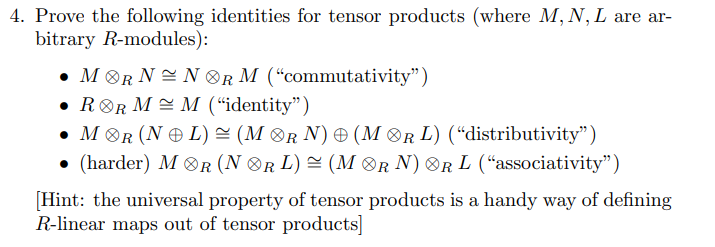
\includegraphics[scale=0.8]{4.png}
	\hfill
\end{problem}

\begin{solution}
\begin{itemize}
\item Consider the map $M \times N \to N \otimes_R M$ given by $((m,n)
\mapsto n \otimes m)$. Notice that this map is $R$-bilinear on $M \times
N$ since $\otimes: M \times N \to M \otimes_R N$ is.
Then by the universal property of tensor products we have a unique
$R$-linear map $f: M \otimes_R N \to N \otimes_R M$ such that $f \circ
\otimes = (m,n) \mapsto n \otimes m$. 
The same argument on the $R$-bilinear map $N \times M \to N \otimes_R
M$ given by $(n,m) \mapsto (m \otimes n)$ gives a unique $R$-linear
map $\tilde f: N \otimes_R M \to M \otimes_R N$ such that\footnote{
The ``$\otimes$'' in the following phrase now refers to the
$R$-bilinear map $N \times M \to N \otimes_R M$, whereas earlier it
referred to the $R$-bilinear map $M \times N \to M \otimes_R N$.
} $\tilde f
\circ \times = (n,m) \mapsto m \otimes n$. 

Notice now that $f \circ \tilde f = id_{N \otimes_R M}$ and $\tilde f
\circ f = id_{M \otimes_R N}$. Indeed $(f \circ \tilde f)(m \otimes n)
= f(n \otimes m) = m \otimes n$. And likewise for the other direction.

That is, we have found a bijective $R$-linear map $M \otimes_R N \to N
\otimes_R M$ and so in fact $M \otimes_R N$ is isomorphic to $N
\otimes_R M$.


\item Consider the following map $M \times N \to M$ via $(r,m) \mapsto
rm$ given by the module structure on $M$. Notice that this map is
bilinear \wg{come back and write the computation out}
And so by the universal property of tensor products we have a unique
$R$-linear map $f: R \otimes_R M \to M$ such that $r \otimes n
\mapsto rm$. 

I claim that this map is bijective and so is an isomorphism of
$R$-modules. First notice that $f$ is surjective. Indeed, if $m \in M$
then $f(1 \otimes m) = 1\cdot m = m$, so long as $R$ is not the zero
ring. If $R$ is the zero ring, then $M$ must be the zero module, and
then our desired isomorphism trivially holds. 

Next we show that $f$ is injective. 
Suppose we have $r \cdot m' = m$ for some $m,m' \in M$ and
$r \in R$. Then notice 
\[
	r \otimes m' = 1 \cdot r \otimes m' = r
		\otimes r \cdot m' = 1 \otimes m,
\]
And so $rm' = m$ implies $r \otimes m' = 1 \otimes m$. This suffices
to show that $f$ is injective because if generally we have $r_1 m_1 =
r_2 m_2$ then by definition $r_1 m_1 = m'$ for some $m' \in M$ and
then we have $m' = r_2 m_2$. 

Overall we have a bijective $R$-linear map $R \otimes_R M \to M$, and
so $R \otimes_R M \cong M$.


\end{itemize}
\end{solution}

\newpage

%------------------------- Problem 5 -----------------------

\begin{problem}[4]
	\hfill
\end{problem}

\begin{solution}
\end{solution}

\newpage

%------------------------- Problem 6 -----------------------

\begin{problem}[4]
	\hfill
\end{problem}

\begin{solution}
\end{solution}

\newpage

%------------------------- Problem 7 -----------------------

\begin{problem}[4]
	\hfill
\end{problem}

\begin{solution}
\end{solution}

\newpage

%------------------------- Problem 8 -----------------------

\begin{problem}[4]
	\hfill
\end{problem}

\begin{solution}
\end{solution}

\newpage

%------------------------- Problem 4 -----------------------

\begin{problem}[4]
	\hfill
\end{problem}

\begin{solution}
\end{solution}

\newpage


\end{document}
